\documentclass[]{article}
\usepackage[a4paper,top=3cm,bottom=2.5cm,left=2.5cm,
            right=2cm,marginparwidth=1.75cm,
            headheight=5pt]{geometry}
\usepackage[T5]{fontenc}
\usepackage[utf8]{inputenc}
\usepackage[document]{}
\usepackage[english]{babel}
\usepackage[unicode]{hyperref}
\usepackage{amsmath}
\usepackage{setspace}
\usepackage{graphicx}
\usepackage{caption}
\usepackage{subcaption}
\usepackage{tcolorbox}
\usepackage{listings}
\usepackage{hyperref}
\usepackage{xcolor}
\usepackage{longtable}
\usepackage{titlesec}
\usepackage{floatrow}
\usepackage[nottoc]{tocbibind}
\usepackage{mdframed}
\usepackage{amsmath}
\usepackage{amssymb}
\usepackage{tgbonum}
\usepackage{type1cm}
\usepackage{indentfirst}
\usepackage{lettrine}
\usepackage{colortbl}
\usepackage{fancyhdr}
\usepackage{wrapfig}
\usepackage{lastpage}
\usepackage{url}
\addto\captionsenglish{
  \renewcommand{\contentsname}{Table of Contents}%
  \renewcommand{\listfigurename}{Danh sách ảnh}%
  \renewcommand{\listtablename}{Danh sách bảng}%
  \renewcommand{\figurename}{Figure}
  \renewcommand{\tablename}{Table}
}
\pagestyle{fancy}
\fancyhf{}
\rhead{Intro to Machine Learning}
\lhead{\color{cyan}Google Data Analytics by Coursera}
\lfoot{Page \thepage /\pageref{LastPage}}
\renewcommand{\footrulewidth}{0.4pt}
\setlength{\parindent}{1.5em}
\setlength{\parskip}{1cm}
\renewcommand{\baselinestretch}{1.5}
\newmdenv[linecolor=black,skipabove=\topsep,skipbelow=\topsep,
leftmargin=2.5cm,rightmargin=2.5cm,
innerleftmargin=5cm,innerrightmargin=5cm]{mybox}
\usepackage{multicol}
\usepackage{indentfirst}
\usepackage{color}
\usepackage{tikz}
\graphicspath{{Figures/}} 
\usepackage{lipsum}
\usetikzlibrary{calc}
\setlength{\columnseprule}{2pt}
\def\columnseprulecolor{\color{black}}
\def\maru#1{\textcircled{\scriptsize#1}}

\usepackage[backend=biber, style=numeric]{biblatex}
\addbibresource{refs.bib} % Tải tệp references.bib
\defbibheading{mybibintoc}{\section{Tài liệu tham khảo}}


\begin{document}

% Bìa trang
\begin{titlepage}
  \begin{tikzpicture}[remember picture,overlay,inner sep=0,outer sep=0]
    \draw[blue!70!black,line width=4pt] ([xshift=-1.5cm,yshift=-2cm]current page.north east) coordinate (A)--([xshift=2cm,yshift=-2cm]current page.north west) coordinate(B)--([xshift=2cm,yshift=2cm]current page.south west) coordinate (C)--([xshift=-1.5cm,yshift=2cm]current page.south east) coordinate(D)--cycle;

    \draw ([yshift=0.5cm,xshift=-0.5cm]A)-- ([yshift=0.5cm,xshift=0.5cm]B)--
    ([yshift=-0.5cm,xshift=0.5cm]B) --([yshift=-0.5cm,xshift=-0.5cm]B)--([yshift=0.5cm,xshift=-0.5cm]C)--([yshift=0.5cm,xshift=0.5cm]C)--([yshift=-0.5cm,xshift=0.5cm]C)-- ([yshift=-0.5cm,xshift=-0.5cm]D)--([yshift=0.5cm,xshift=-0.5cm]D)--([yshift=0.5cm,xshift=0.5cm]D)--([yshift=-0.5cm,xshift=0.5cm]A)--([yshift=-0.5cm,xshift=-0.5cm]A)--([yshift=0.5cm,xshift=-0.5cm]A);


    \draw ([yshift=-0.3cm,xshift=0.3cm]A)-- ([yshift=-0.3cm,xshift=-0.3cm]B)--
    ([yshift=0.3cm,xshift=-0.3cm]B) --([yshift=0.3cm,xshift=0.3cm]B)--([yshift=-0.3cm,xshift=0.3cm]C)--([yshift=-0.3cm,xshift=-0.3cm]C)--([yshift=0.3cm,xshift=-0.3cm]C)-- ([yshift=0.3cm,xshift=0.3cm]D)--([yshift=-0.3cm,xshift=0.3cm]D)--([yshift=-0.3cm,xshift=-0.3cm]D)--([yshift=0.3cm,xshift=-0.3cm]A)--([yshift=0.3cm,xshift=0.3cm]A)--([yshift=-0.3cm,xshift=0.3cm]A);

  \end{tikzpicture}
  \newcommand{\HRule}{\rule{\linewidth}{0.5mm}}
  \center

  \textsc{\Large UNIVERSITY OF SCIENCE}\\[0.5cm]
  \textsc{\Large FACULTY OF INFORMATION TECHNOLOGY}\\[1cm]
  
\includegraphics[width=0.3\textwidth]{logo/KHTN.jpg}\\[1cm]

  \HRule \\[0.4cm]
  {\huge \bfseries GOOGLE DATA ANALYTICS} \\[0.4cm]
  {\large COURSERA}\\[0.1cm]
  \HRule \\[1.5cm]

  \centerline{\Large{\textbf{Triệu Nhật Minh — 21127112 — 21KHMT2}}}
  \vspace{2.5cm}
  \centerline{\large{\textit{Giảng viên hướng dẫn}}}
  \vspace{0.25cm}
  \centerline{\large{Bùi Duy Đăng}}
  \centerline{\large{Phạm Trọng Nghĩa}}
  \centerline{\large{Nguyễn Ngọc Đức}}
  \vspace{3cm}
  \centerline{\today}


  \vfill % Wipe blank space of the page.
\end{titlepage}

% Mục lục tự động
\setlength{\parskip}{.7em}
\tableofcontents
\newpage

% Table of Figures & Tables
\setlength{\parskip}{.5em}
%\listoffigures
%\listoftables
\newpage

% Bắt đầu nội dung

\section{Preface}
\subsection{About this course}
I am grateful for the opportunity to be one of the recipients of the 2022 Digital Talent Scholarship funded by NIC. This scholarship has enabled me to pursue my passion for data science and enhance my skills in this field. One of the remarkable features of this scholarship is that it is still active, which means I can continue to access various online courses. I have chosen to take the Google Data Analytics. In this report, I will share my opinions with the certificate and the course challenge.
\section{Certificate}
\subsection{Professional Certificate: Google Data Analytics by Coursera}
\begin{figure}[ht!]
  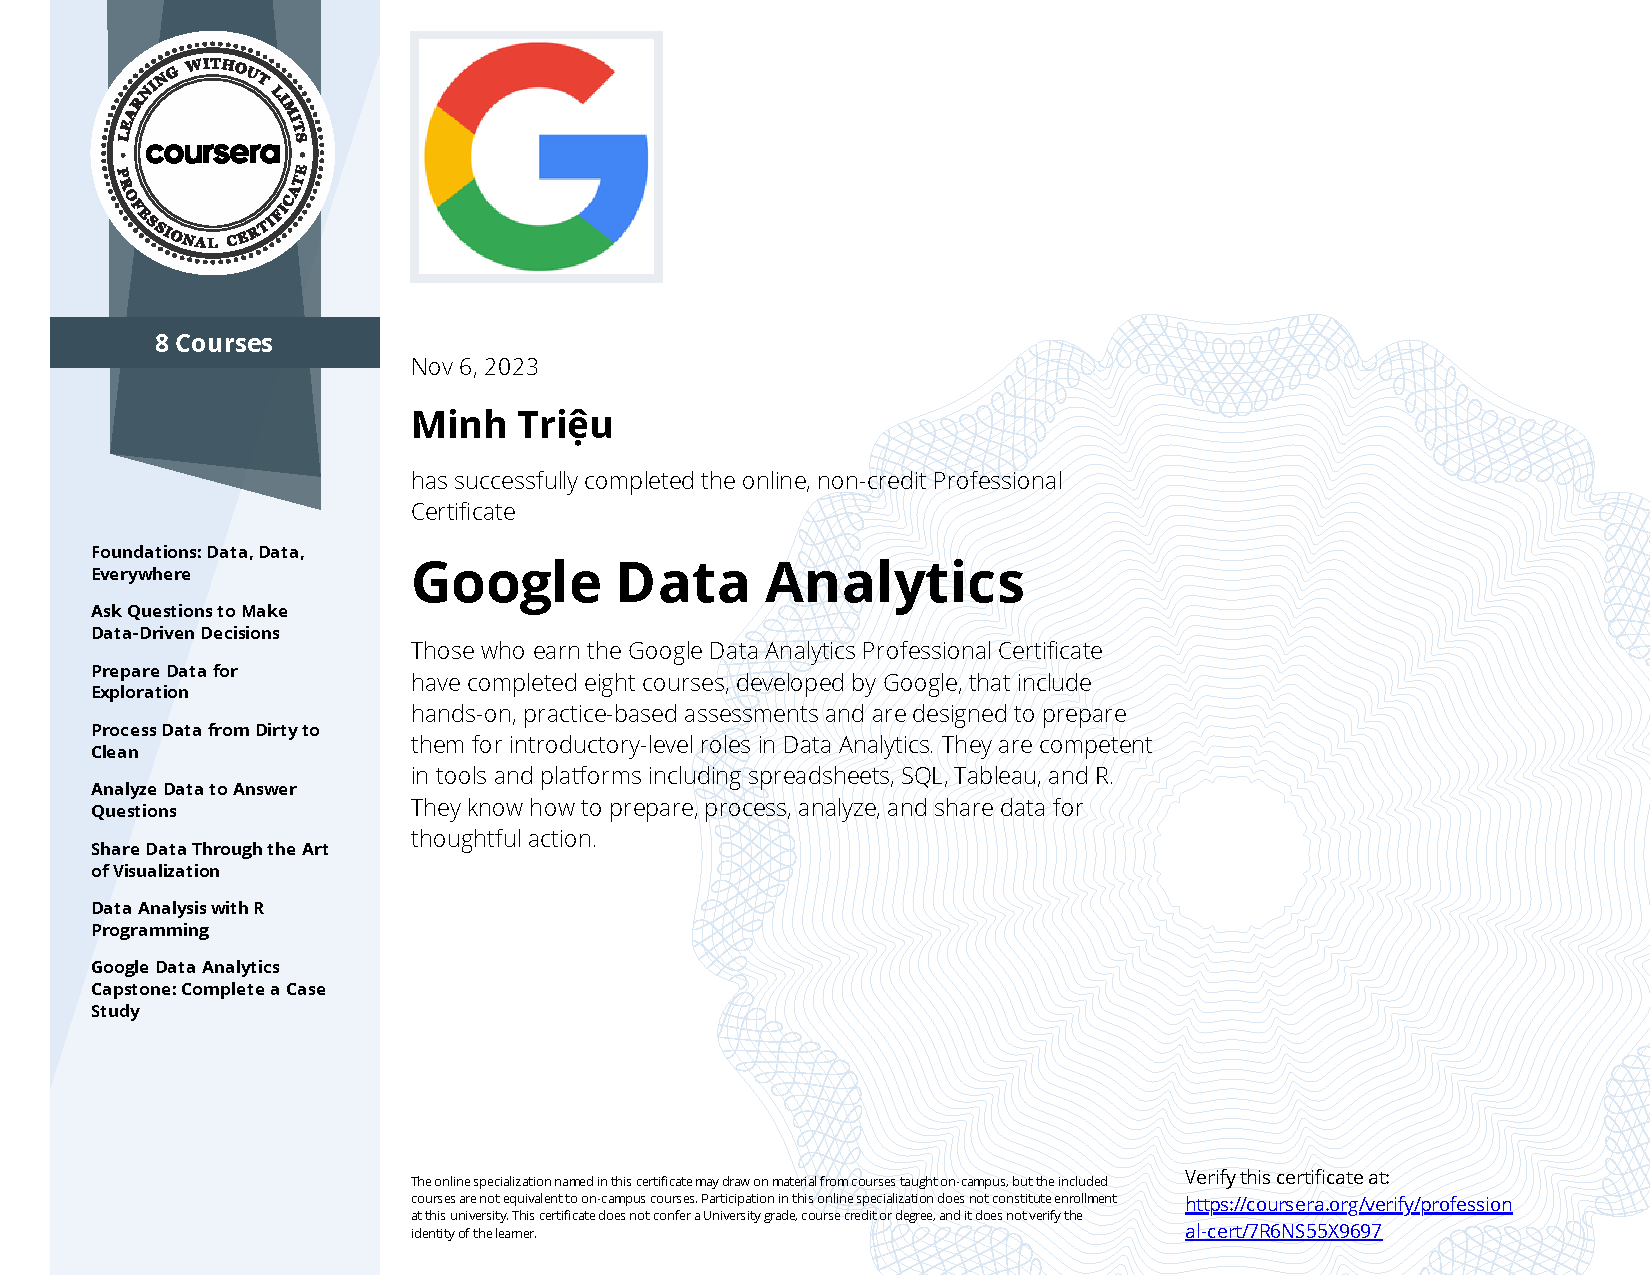
\includegraphics[width=\textwidth]{certs/7R6NS55X9697.pdf}
  \caption{\href{https://www.coursera.org/account/accomplishments/specialization/certificate/7R6NS55X9697}{Verification}}
\end{figure}

\subsection{Enrollment date (8 courses)}
\begin{enumerate}
  \item \href{https://www.coursera.org/account/accomplishments/certificate/S9CWWMGFJAMM}{Foundations: Data, Data, Everywhere - 22nd October 2023}
  \item \href{https://www.coursera.org/account/accomplishments/certificate/ZA7TH6KEEEPB}{Ask Questions to Make Data-Driven Decisions - 24th October 2023}
  \item \href{https://www.coursera.org/account/accomplishments/certificate/B7PZ38G3U9XR}{Prepare Data for Exploration - 27th October 2023}
  \item \href{https://www.coursera.org/account/accomplishments/certificate/DYHS63889XUN}{Process Data from Dirty to Clean - 29th October 2023}
  \item \href{https://www.coursera.org/account/accomplishments/certificate/6478SYGTR4HF}{Analyze Data to Answer Questions - 5th November 2023}
  \item \href{https://www.coursera.org/account/accomplishments/certificate/8JULNPUM3GLC}{Share Data Through the Art of Visualization - 6th November 2023}
  \item \href{https://www.coursera.org/account/accomplishments/certificate/JPHDNMYYDJZ9}{Data Analysis with R Programming - 6th November 2023}
  \item \href{https://www.coursera.org/account/accomplishments/certificate/7TN58662AD9X}{Google Data Analytics Capstone: Complete a Case Study - 6th November 2023}
\end{enumerate}
Completion date of each course: On certificate verification link.

\section{Course 1: Foundations: Data, Data, Everywhere}
I have gained a lot of knowledge from the course. It has taught me how to turn data into insights and comprehend the data ecosystem. I have also learned how to use data to make informed business decisions.
In module 2, I have developed my data analyst skills and practiced analytical thinking. I have learned how to define outcomes and how to measure them. I have also learned how to formulate good questions and communicate effectively with data.\par
In module 3, I have followed the data life cycle and described the data analysis process. I have learned about the data analysis toolbox and how to apply different tools for different tasks. I have also learned how to clean, explore, analyze, and interpret data.\par
In module 4, I have mastered spreadsheet basics and SQL. I have learned how to manipulate, query, and join data using spreadsheets and SQL. I have also learned how to plan a data visualization and select the right chart type for my data.\par
In module 5, I have explored data analyst job opportunities and the importance of fair business decisions. I have learned how to prepare for a data analyst interview and showcase my portfolio. I have also learned how to avoid bias and ensure ethical use of data. This course has provided me with a solid foundation for becoming a data analyst. I have learned how to use data to make informed business decisions. I have also learned how to use spreadsheets and SQL for data analysis.\par
About module challenges and course challenge, I find them very interesting and useful. They have helped me to practice my data analyst skills and apply what I have learned in the course. The instructor emphasizes the importance of asking questions and not making assumptions in data analysis work. He shared a story about an analyst who initially struggled because he was afraid to ask questions, but improved significantly once he started doing so.

\section{Course 2: Ask Questions to Make Data-Driven Decisions}
In the first module, I've gained knowledge on how to leverage data as a problem-solving tool and the art of formulating effective questions to guide my analysis. Furthermore, I've been introduced to the six stages of data analysis: ask, prepare, process, analyze, share, and act and acknowledged. I've also learned that data analysts commonly deal with six types of problems: making predictions, classifying things, detecting anomalies, identifying themes, uncovering relationships, and recognizing patterns.\par

In the second module, I've learned how to effectively communicate my findings through clear and engaging visuals. I've understood the difference between data and metrics, and how to choose the right metrics for my analysis. I've also gained knowledge on how to design compelling dashboards that can summarize my data, highlight key insights, and tell a story. Through practice quizzes, I've tested my knowledge on following the evidence and designing dashboards. The final task of the module helped me assess my understanding of the content and my ability to connect the data dots. Overall, this module has significantly enhanced my skills in data visualization and communication.\par

The third module taught me how to work with spreadsheets, which are essential tools for data analysis. It showed me how to use formulas and functions to perform calculations and manipulate data. It also demonstrated how to save time with structured thinking by using tables, filters, sorting, and conditional formatting. Even though I had used spreadsheets before, I learned many new things from this module. For instance, I used to struggle with the VLOOKUP function, but now, thanks to the hands-on activity, I can use it with ease.\par

The fourth module enhanced my data analyst communication skills. I learned to present data analysis results clearly using suitable visualizations and language. I practiced tailoring my messages to different audiences and responding to various data scenarios. The module also taught me to balance project expectations by setting SMART objectives, defining scope and deliverables, and transparently communicating progress and challenges. I learned to handle the tradeoff between speed and accuracy in data analysis, understanding data uncertainties and limitations.\par

\section{Course 3: Prepare Data for Exploration}


\section{Course 4: Process Data from Dirty to Clean}
\begin{itemize}
  \item
\end{itemize}
\section{Course 5: Analyze Data to Answer Questions}
\begin{itemize}
  \item
\end{itemize}
\section{Course 6: Share Data Through the Art of Visualization}
\begin{itemize}
  \item
\end{itemize}
\section{Course 7: Data Analysis with R Programming}
\begin{itemize}
  \item
\end{itemize}
\section{Course 8: Google Data Analytics Capstone: Complete a Case Study}
\begin{itemize}
  \item
\end{itemize}
\section{Conclusion}
\begin{itemize}
  \item
\end{itemize}
\end{document}